\chapter{Concept}
\section{Common Defenitions and Representations}
\subsection{Definition of the Configuration Space}
As the exact representation of our objects should not matter, we will only define the common points needed for a clear communication of the stated problem.\\
The algorithms aim is to tell if there is a solution possible and, if so, present it. The object which needs to be moved from a starting configuration to a target configuration will be named main object M. Other movable objects are obstacles named $Ob_i$  and the stationary objects are called rims $R_i$. This will be combined to the sets $O = \{M\}  \cup \{Ob_i | i \in \mathbb{N} \} $ and $ R = \{ R_i | i \in \mathbb{N}\}$.\\

Each object $O_A$ contains some data for representing its shape stored under $O_A$.data. Furthermore the configuration of $O_A$ is given by the vector $(x_A,y_A,\phi_A)$ and stored under $O_A$.mid as the middle/reference point for said object where $x_A$ and $y_A$ gives the point around which the object will be rotated by $\phi_A$.
By substraction of the first two dimensions occupied by R from the possible space $O_i$ per object in O, and, if we divide the space in two, selecting the one in which $O_i.mid$ is located at the start, we get a valid space $C_{O_i-R}$ for the object $O_i$ to be moved in ( not taking into account other objects). This space is a simple 3 dimensional space with $x_i, y_i$ and $\phi_i$ as base.\\
But as there is the need to check for collision with ALL other objects $O' = \{O_j, | j\neq i \wedge j \in \mathbb{N}\} $ we need to increase the dimensions of all spaces $C_{O_i-R}$ by the number of objects in $O'$. Also for each set $j$ of dimensions $(x_j,y_j,\phi_j)$  added, we will need to substract the current position of the corresponding object $O_j$ from the space, such that all collision points are removed from $C_{O_i-R}$. This will give us the configuration space for object $O_i$, $C_{O_i}$.


\subsection{Building the Configuration Space}
\label{subsec:confspace}
To build such a configuration space, every possible configuration of every movable object needs to be calculated. Even those who are NOT valid need to be computed at least once, to check if they are valid or not.\\
Each object A has three dimensions $(x_A,y_A,\phi_A)$, with $x$ and $y$ beeing a finite range from $r_x=[x_l, x_h]$ and $r_y=[y_l, y_h]$ defined by the stationary rims of the riddle. The rotation component $\phi$ is choosen from a set of angles $\Phi = \{ \phi | \phi \in r_\phi=[1, 360] \}$. As this would lead to an infinite amount of possible $x,y$ and $\phi$, we could allow steps only, e.g. $x,y,\phi \in \mathbb{N}$.\\
If there are n movable objects we get a total number of possible combinations in the range of $(r_x\cdot r_y \cdot r_\phi )^n$.
Under the premise of saving every calculated combination so that we only calculate each set once and assuming that the time $t_s$ needed for collision check and calculating one set is constant, we get the following formula for the time to calculate the complete configuration space.
\begin{align*}
 T_conf = (r_x\cdot r_y \cdot r_\phi )^n \cdot t_s
\end{align*}
Now we define $t_s = 0.1 ms$ set $r_x = r_y = 10$ and $r_\phi = 180$ with only two objects ( one main object M one obstacle O) meaning $n=2$ we get
\begin{align*}
T_conf &= (10*10*180)^2 \cdot 0.1ms\\
	&=   324000000 \cdot 0.1 ms\\
	&= 3.24 \cdot 10^7 \cdot ms
	&= 9 h
\end{align*} 
This means we would need to wait 9h to completely calculate all possible positions on a very raw grid ( each step just 1 unit) without even having started to search on it.

So the idea is to interleave search and building of the configuration space in such a way, that only the needed nodes are calculated and checked.
But still this would be very slow if we consider implementing it on such a grid. Therefore another approach is needed.\\


\subsection{Dividing the Space in Cells}
\label{subsec::cells}
Instead of taking a grid, the configuration space is divided into cells depending on the current positition of the objects. This cell division will heavily decrease the number of search nodes in the space. The drawback on the other hand is, that this division is dependent on the object representation. So instead of computing an independent configuration space for the search, the search needs to use some information from the objects. Thus a combination of a set of collision information for each point in the configuration space is calculated for each search step. This will lead to an integration of search algorithm and object representation into one main algorithm.\\
\begin{figure}[H]
\centering
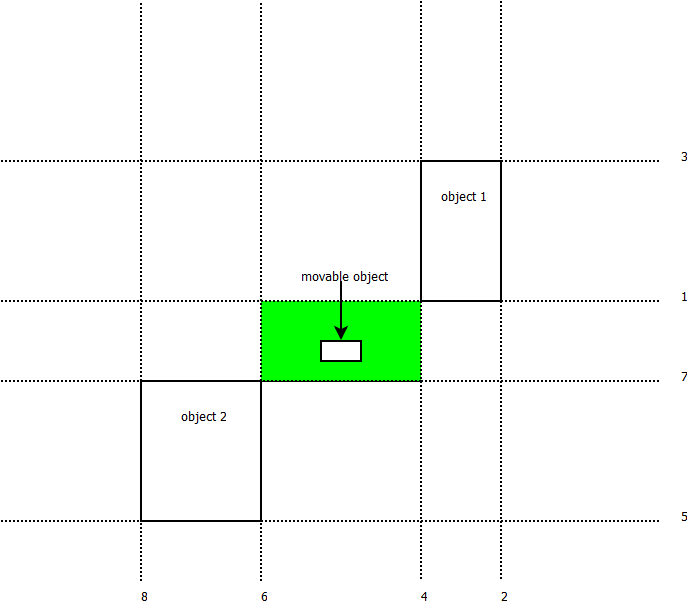
\includegraphics[scale=0.5]{cellDivision}
\caption{Figure showing two objects and their extended borders}
\label{cellDivision}
\end{figure}
So to identify in which cell a point $p$ is in, one takes the borders of each object and extends them beyond their normal length. Doing so will split the space in 2 for each border extended. So if we say we have $n$ borders to extend, we can check if the point $p$ is under/over ( right/left ) of those borders, leading to a binary vector with each position being $1$ if $p$ is over the border, $0$ otherwise. This vector can be seen as a binary number, thus each cell on the plane can be identified by a single number $I$. In figure \ref{cellDivision} the moving objects binary vector would be $(0 1 0 1 1 1 1 1) =  95$.\\
This only works for one point on an otherwise static field, so for each moving object, their cell position needs to be calculated seperatly. Also rotations propose a problem, because the borders of an rotated object may change the cells, but they dont need to. So if there is the need to rotate an object, there is no telling the difference beetween object $O_1$ with configuration $(x,y,0)$ and $O_2$ with configuration $(x,y,1)$ if the cells for all moving objects stay the same.\\
Thus each possible rotation $\phi_i$ for each moving object $O_i$ with $i \in \mathbb{N} \wedge i \leq n$ is taken into account by adding their value to the cell identifier. One configuration can then be seen as $(I_1 , I_2,...,I_n,\phi_1,\phi_2,..,\phi_n)$.\\
The exact way of checking for borders to get a simple search graph depends on the implementation. In the following part two ways of representing the objects will be used.


\subsection{Objects as Point List}
\label{subsec::pointlist}
One of the possible ways of describing an object in a two dimensional setting would be an ordered list of corner points.  Together with an anchor point we can calculate all transformations needed.
\subsubsection{Main steps}
To see if this representation would work we take a short look at the algorithm described in \ref{sec:Idea} and sketch a solution to each step.
\begin{enumerate}
\item Generate $C_{O_i-R}$:By identifying the main outer rim $R_mo$ and computing its inner hull for $O_i$ the space $C_{O_i}$ is build. For all other rims $R_j$ computing the convex hull with $O_i$ and substracting them from $C_{O_i}$ leads to $C_{O_i-R}$.
\item Generate $C_{O_i-O_j}$: Calculate the convex hull from $O_i$ to each other object $O_j$.
\item Generate $C_{O_i}$: Substraction of $C_{O_i-R} - C_{O_i-O_j}$ for all $O_j \in O \wedge j \neq i$.
\item Divide search space in cells: By extending the vectors connecting the convex hull in $C_{O_i-O_j}$ we get a seperation of the space in $C_{O_i}$ in multiple parts. Each step is a translation of the object $O_i$  from one cell to another. The neighbour cells can be identified by iterating over the objects $O_j$ and calculating the nearest crossing along $(x,y)$ with the extended vectors of its convex hull. \\ Rotations are represented as a jump from one hyperplane to the next in search direction. There are multiple problems with rotation in this representation, that will be discussed later.
\item Construct the search graph: While moving along those cells, we adapt $C_{O_i}$ for each $O_i \in O$ each step. These cells are then added to the graph.
\item Search for target: Again independently of the object representation a search can then be applied to the resulting graph. 
\end{enumerate}


So far this representation seems like a good choice in multiple ways with some drawbacks on the other hand.\\
Pros:
\begin{itemize}
\item Simple and intuitive representation of object itself
\item Easy and fast to compute concerning the transformation of an object (translation, rotation)
\end{itemize}
Cons:
\begin{itemize}
\item Rotation needs discrete steps along the config dimensions $\phi_i$, therefore more exact calculations lead to higher need in computation power.
\item The more corners an object has, the more points its convex hull with other object will have. One point more in object $O_i$ can lead to $n$ more points in $C_{O_i-O_j}$ with $n$ beeing the number of points in $O_j$. As we use the vectors connecting the points in $C_{O_i-O_j}$, $n$ more cells will arise in the search space due to those ghost planes.
\end{itemize}

In the following this algorithm will be named pList.


\subsection{Objects as Function List}
\label{subsec:functionlist}
Another option of describing an object is the representation with functions and definition ranges. Each function is then represented as a list of coefficients $a,b,c$ describing the polynom $ax^2 + bx + c$. Also an anchor point as a reference is needed for rotating the object.\\

\subsubsection{Main steps}
The algorithm slightly changes for this representation, solving problems that existed with the point list representation, but introducing new ones. One step of moving an object in one direction would be described as follows:
\begin{enumerate}
\item The object $O_i$ is moved function by function. So for each function $f_{o_i}$ describing a border, this function will be moved in the searching direction. By eliminating all functions that are not in the way by looking at the definition/value ranges, a lot of computing time is saved.\\ 
Iterating over all other objects $O_j \in O \wedge j \neq i$ and their functions $f_{o_j}$ and solving $f_{o_i} = f_{o_j}$ then yields a solution with information about the distance in search direction. The new configuration for the object $O_i$ can then be computed.
\item The function with the minimal distance to the object is saved as the closest function together with the new configuration. If no function could be found, the object is moved to the border in the searching direction.
\item The whole object will then be transformed according to the configuration saved, or if the object is already able to be moved to the target configuration in a direct line, the program ends. This is done by connection each corner of the main object with the target area and checking those functions for intersection.
\end{enumerate}

As noted, this representation solves some problems from the previous one but still carries some drawbacks.\\
Pros:
\begin{itemize}
\item The collision set of a point in the configuration space does not need to be computed, as it is defined directly by the anchor points of the objects itself. The outer rim $R_{mo}$ is considered seperate from the objects. Each non-moving object is treated just like a normal object, only that its anchorpoints values in the configuration space along $x,y$ and $\phi$ are constant.
\item With the ability to get rid of functions that are not in the way, the number of search cells goes down due to the absence of ghost planes.
\end{itemize}
Cons:
\begin{itemize}
\item Having direct points in the config space can lead to multiple nodes in the graph due to small movements that would normaly be compromised by cell representation.
\item There is no direct way to represent a vertical line with a function. A workaround is to use a function with a extremly high gradient inside a small definition range.
The problem is that this can lead to computational errors due to the fact that the optimal gradient would be infinite.
\item Rotation still needs discrete steps along the config dimensions $\phi_i$, Therefore more exact calculations lead to higher need in computation power.
\end{itemize}

In the following this algorithm will be known as fList.

\subsubsection{Adaption Using Cells as Sodes}
As proposed in \ref{subsec::cells} an adaption to the algorithm $fList$ has been made in a way, that the ghostplanes still dont interfere with the movement of the objects, but the number of search nodes in the graph decrease for few object in the riddle.\\
To do so, each point that has been found a valid next step checked for its cell. This cell information is then used as the next node in the search graph. If another step lands in the same cell, the two different positions in the cell are evaluated, and if necessery updated according to the given heuristic, to change the cells distance value to the target.This way all points in the cell amount to the same node in the graph, thus getting rid of many small movement changes.\\
The drawback on the other hand is, that for many objects in the riddle, the amount of existing cells can lead to unnecessary updates and thus unnecessary movements as the algorithm jumps back to a previous node that now has a better value.\\ 
In the following this algorithm will be know as fCell.